\chapter{Resolution of names}
The following section will talk about history of technologies under the resolution of server names in URL to their IP addresses, needed to extablish the connection.

\section{Network Information Center (NIC)}\label{NIC_section}
This type of architecture was used in the past to resolve names. Each client has its own file \textbf{HOSTS.txt}, with resolution of names. The client shared its file with a central system, called \textbf{NIC} (Figure \ref{NIC}). This system collects all the files, like an hub, and shared resolution names to other clients.\\
This architecture is unfeasable and not scalable with nowadays number of IP addresses, because the files become very huge and transfering becomes very slow.\\
\begin{figure}[h]
\centering
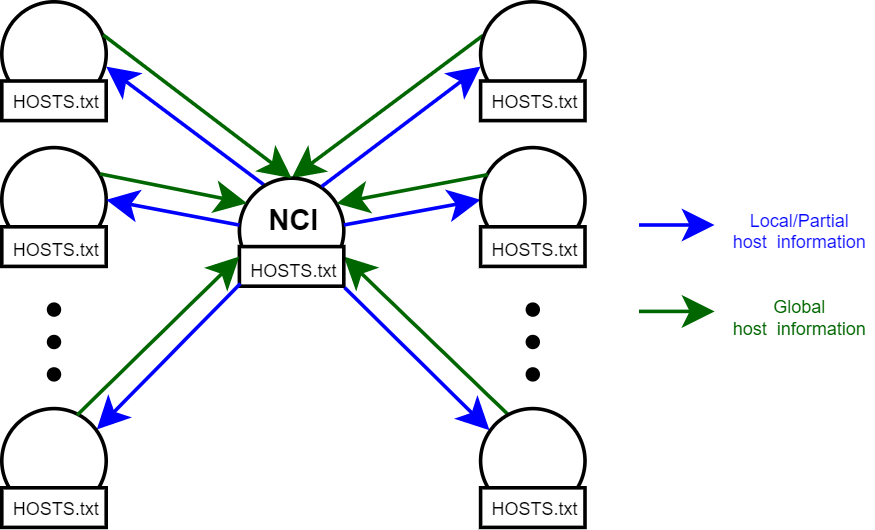
\includegraphics[scale=0.4]{Images/Resolution/NIC}
\caption{\footnotesize{How NIC worked.}}\label{NIC}
\end{figure}


\section{Domain Name System (DNS)}\label{DNS_system}
The file \textbf{HOSTS.txt} is yet used in nowadays UNIX systems (Section \ref{NIC_section}). The specified host name is searched in local \textbf{/etc/hosts.txt}, that contains local and private addresses resolution table, and if not found, it will be searched through DNS\cite{RFC1034}.

\subsection{Goals}
\begin{enumerate}
\item{Names should not be required to contain network identifiers, addresses, routes, or similar information as part of the name.}
\item{The sheer size of the database and frequency of updates suggest that it must be maintained in a distributed manner, with local caching to improve performance.\\
Approaches that attempt to collect a consistent copy of the entire database will become more and more expensive and difficult, and hence should be avoided.\\
The same principle holds for the structure of the name space, and in particular mechanisms for creating and deleting names; these should also be distributed.}
\item{Where there are tradeoffs between the cost of acquiring data, the speed of updates, and the accuracy of caches, the source of the data should control the tradeoff.}
\item{The costs of implementing such a facility dictate that it be generally useful, and not restricted to a single application.\\
We should be able to use names to retrieve host addresses, mailbox data, and other as yet undetermined information. All data associated with a name is tagged with a type, and queries can be limited to a single type.}
\item{Because we want the name space to be useful in dissimilar networks and applications, we provide the ability to use the same name space with different protocol families or management.\\
For example, host address formats differ between protocols, though all protocols have the notion of address. The DNS tags all data with a class as well as the type, so that we can allow parallel use of different formats for data of type address.}
\item{We want name server transactions to be independent of the communications system that carries them.\\
Some systems may wish to use datagrams for queries and responses and only establish virtual circuits for transactions that need the reliability (e.g., database updates, long transactions); other systems will use virtual circuits exclusively.}
\item{The system should be useful across a wide spectrum of host capabilities.\\
Both personal computers and large timeshared hosts should be able to use the system, though perhaps in different ways.}
\end{enumerate}

\subsection{Hierarchy structure}
Hierarchy permits to manage a lot of nambers of domain names and IP addresses, reducing the time spent to resolve them. Given for example the host name \textbf{www.dei.unipd.it}, we have a \textbf{Name Server (NS)} for each of the domain name inside it (Figure \ref{DNS_hierarchy}). The tree hierarchy has a name server for each one of its internal nodes.The name server gives us only the name of the name server of the lower level to which we need to go.\\
To obtain the IP address of this name server, we need to ask, to name server of upper layer, a \textbf{glue record}. The glue record is an additional information that is needed by us to understand how to reach that name server. Hence the glue record is the IP address of NS of the lower level in hierarchy. \\
For each request to NS, we obtain also the expiration time information because a caching approach is adopted in DNS but at level 4. There are 13 root name servers that are obtained when asking resolution to root. \\
In reality root name servers are more than 13 but the communication used in DNS is made through UDP and this type of connection supports only 13 simultaneously transfers. The local DNS server for the device, managed by my network provider, contains the 13 root servers and permits us to reach at least one DNS root server.\\
The 13 DNS root servers are added locally during the installation of local DNSs and updated assuming that at least one root server of them can be reachable. There is no address record for the root.\\
In general structure of the queries to name servers, we ask only the resolution for a specific domain that composes the whole name (Figure \ref{default_DNS}).\\
To use a caching system efficiently, we need to make a recursive query, sending the request of resolution of the whole name with all its domains (Figure \ref{recursive_DNS}). All the name servers, where the query passes throuh, store information about resolution. This system is never applied as it is.\\
In reality an hybrid version is implemented, using only partial recursion (Figure \ref{hybrid_DNS}). Local DNS usually has huge cache with main important names and also first and second level have caches. So local DNS rarely asks resolution to TOP Level Domain or Root.\\
Recursive query option in dig command is made by a flag, default set to yes and used in UDP packet as an additional information. The Root Name Server decides if it wants to accept recursive query or if not, how many domains can resolve. I can group some domains, defining a zone, so I can use only a name server for a specific zone to solve many domains together (Figure \ref{DNS_zone}). So the name servers are authorithative over zones and not only single domains.\\
The creation of the zones are used to manage easily the responsability of companies and their organization over the zones, grouping domains. Another reason for this partition in zones is the presence of some domains with few names, that it's better to group with other domains.
\begin{figure}[h]
\centering
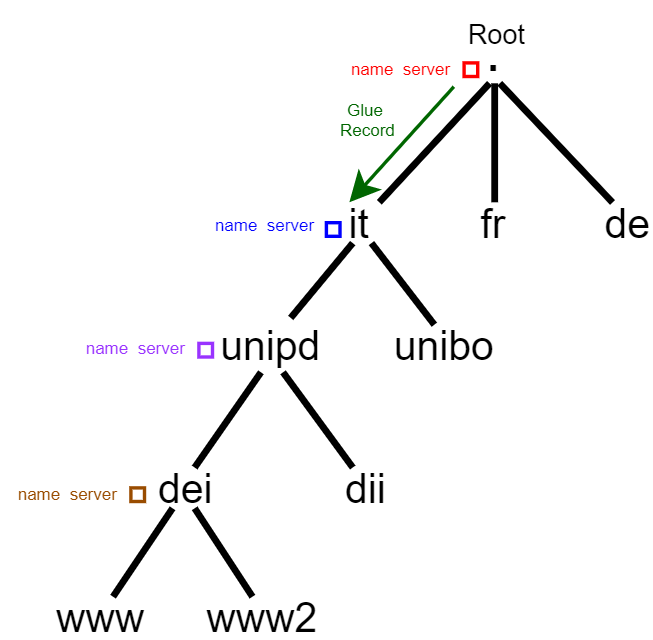
\includegraphics[scale=0.38]{Images/Resolution/DNS_hierarchy}
\caption{\footnotesize{DNS structure.}}\label{DNS_hierarchy}
\end{figure}
\begin{lstlisting}[linewidth=470pt, style=code, caption=Example of default DNS queries using dig.]
//Ask for root name server to the default name server 
dig -t NS -n .
 
//Ask for address of root name server "a.root-servers.net", previously chosen
dig -t A -n a.root-servers.net 

//Ask for "it" name server to the "a.root-servers.net" address, previously chosen
dig @198.41.0.4 -t NS it 

//Ask for address of "nameserver.cnr.it" name server,  previously chosen for "it" domain
dig @198.41.0.4 -t A  nameserver.cnr.it

//Ask for "unipd.it" name server to the "nameserver.cnr.it" address 
dig @194.119.192.34 -t NS -n unipd.it

//Ask for "unipd.it" name server to the "nameserver.cnr.it" address 
dig @194.119.192.34 -t A unipd.it

//Ask for "dei.unipd.it" name server to one ("mail.dei.unipd.it" 
dig @147.162.1.100 -t NS  dei.unipd.it

//Ask for address of "mail.dei.unipd.it" name server, previously chosen 
dig @147.162.1.2 -t A  mail.dei.unipd.it 

//Ask for address of "www.dei.unipd.it" to "mail.dei.unpd.it" name server, previousy chosen 
dig @147.162.2.100 -t A  www.dei.unipd.it
\end{lstlisting} 
\begin{figure}[h]
\centering
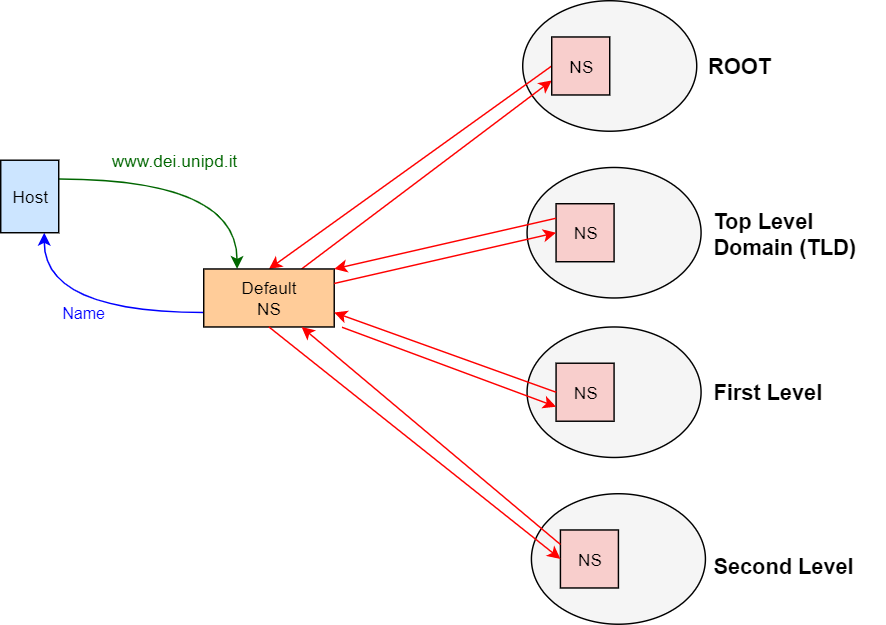
\includegraphics[scale=0.4]{Images/Resolution/default_DNS}
\caption{\footnotesize{Default DNS behaviour without caching.}}\label{default_DNS}
\end{figure}
\begin{figure}[h]
\centering
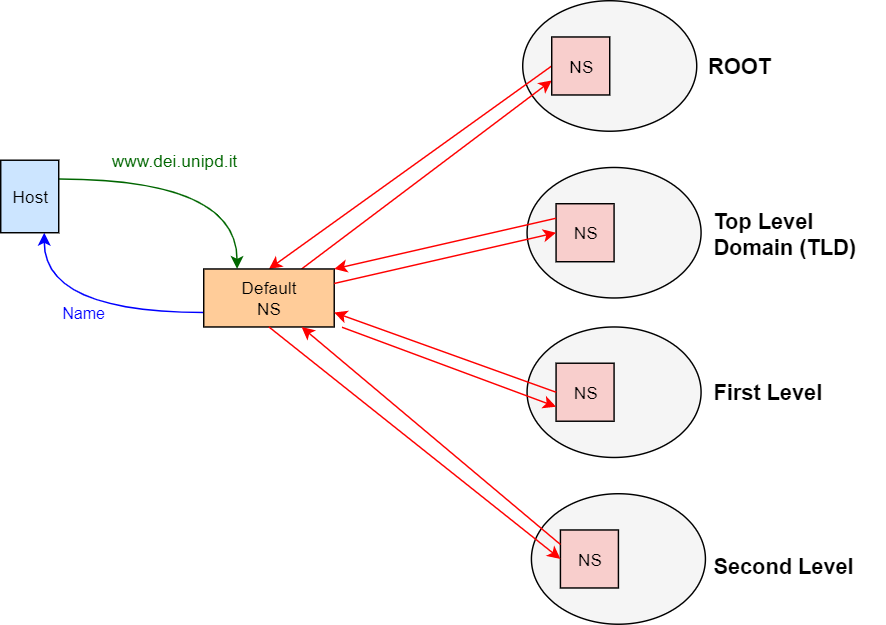
\includegraphics[scale=0.4]{Images/Resolution/default_DNS}
\caption{\footnotesize{Completely recursive DNS structure.}}\label{recursive_DNS}
\end{figure}
\begin{figure}[h]
\centering
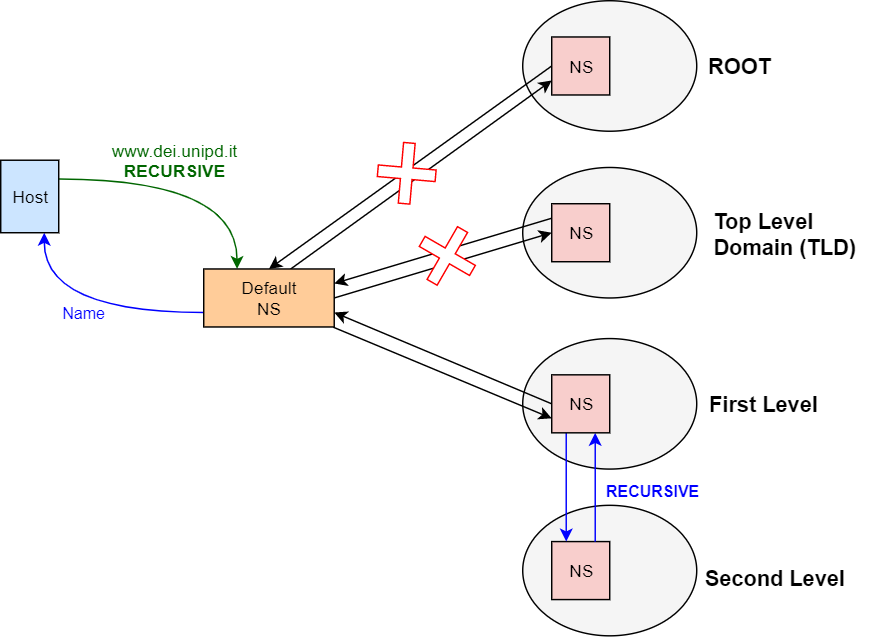
\includegraphics[scale=0.4]{Images/Resolution/hybrid_DNS}
\caption{\footnotesize{Hybrid DNS structure.}}\label{hybrid_DNS}
\end{figure}
\begin{figure}[H]
\centering
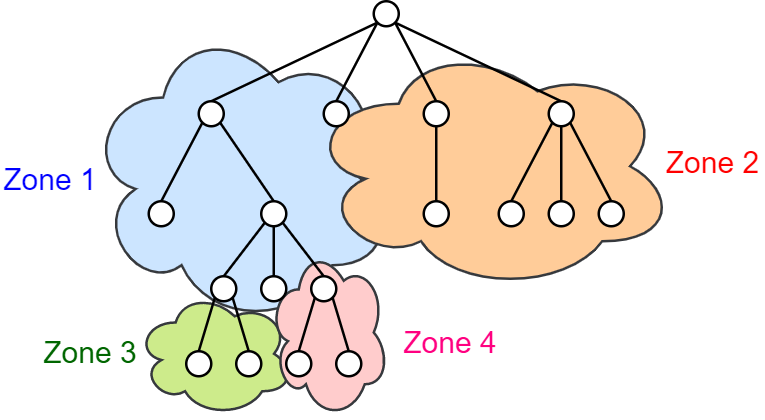
\includegraphics[scale=0.4]{Images/Resolution/DNS_zone}
\caption{\footnotesize{Example of partitioning into zones.}}\label{DNS_zone}
\end{figure}